% !TeX root = booklet-01.tex
\section{گیت‌های ایستای \lr{CMOS}}
\label{sec:book-cmos}
\label{sec:ch1-static}
\subsection{شبکه بالا و پایین چه وظیفه‌ای دارند؟}
گیت \lr{Static Complementary CMOS} یک شبکه \lr{pMOS} میان تغذیه و خروجی
به نام \lr{Pull-up Network (PUN)} و یک شبکه \lr{nMOS} میان خروجی و زمین
به نام \lr{Pull-down Network (PDN)} دارد.
برای ورودی‌های دودویی پایدار و در مدل \lr{Switch}، باید دقیقاً یکی از دو شبکه
مسیر برقرار داشته باشد \cite[بخش \secnum{۱.۴.۳}]{weste}.
این «دقیقاً یکی» هم از خروجی شناور و هم از مسیر مستقیم تغذیه به زمین جلوگیری می‌کند.

اگر شرط هدایت پایین را \(F\) بنامیم، خروجی وقتی \(F=1\) است صفر می‌شود.
پس \(Y=\overline{F}\)، و شبکه بالا باید شرط \(\overline{F}\) را پیاده کند.
\textbf{شرط هدایت شبکه پایین را نباید با تابع خروجی یکی گرفت.}
جدول \ref{tab:ch1-drive} چهار حالت کلی اتصال را نشان می‌دهد.
\begin{table}[ht]
\centering
\caption{حالت خروجی از روی هدایت دو شبکه در مدل مقدماتی؛ اثر گذرا و نشتی حذف شده است.}
\label{tab:ch1-drive}
\begin{tabular}{ccc}
\toprule
شبکه بالا & شبکه پایین & وضعیت خروجی\\
\midrule
قطع & وصل & صفر منطقی\\
وصل & قطع & یک منطقی\\
قطع & قطع & \lr{High Impedance} یا \(Z\)\\
وصل & وصل & \lr{Contention}\\
\bottomrule
\end{tabular}
\end{table}
در \(Z\)، خروجی از دو ریل جداست و مقدار آن ممکن است به بار قبلی وابسته باشد.
در \lr{Contention}، دو شبکه با هم خروجی را به دو ریل می‌کشند؛
مدل کلید ایدئال ولتاژ و جریان واقعی این اتصال را تعیین نمی‌کند.
نماد \(X\) در بحث مدار می‌تواند خروجی نامعین را نشان دهد؛
در جدول فشرده یک تابع، ممکن است به معنی «مقدار ورودی برای این سطر اهمیتی ندارد» باشد.
این دو کاربرد باید از متن تشخیص داده شوند \cite[صفحه چاپی ۱۰ و جدول بخش \secnum{۱.۴.۸}]{weste}.

\subsection{\lr{Inverter}: تحلیل اتصال، نه حفظ جدول}
در شکل \ref{fig:ch1-inverter}، ورودی \(A\) به \lr{Gate} هر دو ترانزیستور
و خروجی \(Y\) به \lr{Drain}های مشترک وصل است.
\lr{Source} بالا به \(V_{\mathrm{DD}}\) و پایین به زمین متصل است؛
بدنه‌ها نیز به‌ترتیب به تغذیه و زمین وصل‌اند و در نماد ساده رسم نشده‌اند.
\begin{figure}[ht]
\centering
\begin{latin}
\begin{circuitikz}[american]
\draw (0,2) node[pmos] (p) {} (0,-1) node[nmos] (n) {};
\draw (p.S)--(0,3.2) node[above] {$V_{\mathrm{DD}}$};
\draw (n.S)--(0,-2.2) node[ground] {};
\draw (p.D)--(0,0.5)--(n.D);
\draw (0,0.5) to[short,*-o] (1.8,0.5) node[right] {$Y$};
\draw (p.G)--(-1.6,2)--(-1.6,-1)--(n.G);
\draw (-1.6,0.5) to[short,*-o] (-2.5,0.5) node[left] {$A$};
\node[right] at (0.5,2) {pMOS};\node[right] at (0.5,-1) {nMOS};
\end{circuitikz}
\end{latin}
\caption{بازترسیم آموزشی \lr{Inverter} بر پایه شکل \secnum{۱.۱۱} کتاب و اسلاید ۲۳
\cite{weste,intro}. حباب \lr{Gate} ترانزیستور بالا نشانه \lr{pMOS} است.}
\label{fig:ch1-inverter}
\end{figure}

اگر \(A=0\)، پایین قطع و بالا وصل است؛ پس خروجی به تغذیه می‌رسد.
اگر \(A=1\)، بالا قطع و پایین وصل است؛ پس خروجی به زمین می‌رسد.
بنابراین \(Y=\overline{A}\). ورودی به خروجی اتصال رسانشی مستقیم ندارد؛
ورودی فقط وضعیت مسیرها را کنترل می‌کند.

اگر خروجی ظرفیت داشته باشد، برای رسیدن به ریل باید شارژ یا دشارژ شود.
از رابطه \(I=C\,\mathrm{d}V/\mathrm{d}t\) در بخش پیش‌نیازها می‌دانیم
این تغییر زمان می‌خواهد. مدل فعلی مقدار منطقی پایدار را می‌دهد، نه زمان گذار.
در ورودی میانی، فرض «دقیقاً یکی روشن است» لزوماً درست نیست؛
تحلیل آن به منحنی انتقال و ناحیه عملکرد جزوه سوم نیاز دارد.

\subsection{\lr{NAND}: سری در پایین، موازی در بالا}
برای دو \lr{nMOS} سری، جریان پایین فقط وقتی مسیر دارد که هر دو ورودی یک باشند؛
پس \(F_{\mathrm{PDN}}=AB\). خروجی در این حالت صفر می‌شود و تابع موردنظر
\(Y=\overline{AB}\) است. طبق \lr{De Morgan}:
\begin{equation}\label{eq:ch1-nand}
F_{\mathrm{PUN}}=\overline{AB}=\overline{A}+\overline{B}.
\end{equation}
هر \lr{pMOS} با صفر ورودی خودش روشن می‌شود، پس شبکه بالا باید دو \lr{pMOS}
موازی داشته باشد. در شکل \ref{fig:ch1-nand-nor}، مسیر هر ورودی را می‌توان دنبال کرد
\cite[بخش \secnum{۱.۴.۲}]{weste}\cite[اسلاید ۲۴]{intro}.

\begin{figure}[ht]
\centering
\begin{latin}
\begin{circuitikz}[american,scale=0.9,transform shape]
\begin{scope}
\draw (0,3) node[pmos] (pa) {} (2,3) node[pmos] (pb) {};
\draw (pa.S)--(0,4)--(2,4)--(pb.S);\node[above] at (1,4) {$V_{\mathrm{DD}}$};
\draw (pa.D)--(0,2)--(2,2)--(pb.D);
\draw (1,0.9) node[nmos] (na) {} (1,-0.8) node[nmos] (nb) {};
\draw (1,2)--(na.D) (na.S)--(nb.D) (nb.S)--(1,-1.8) node[ground] {};
\draw (2,2) to[short,*-o] (3,2) node[right] {$Y$};
\node[left] at (pa.G) {$A$};\node[left] at (pb.G) {$B$};
\node[left] at (na.G) {$A$};\node[left] at (nb.G) {$B$};
\node at (1,-2.5) {NAND};
\end{scope}
\begin{scope}[xshift=7cm]
\draw (1,3) node[pmos] (pc) {} (1,1.3) node[pmos] (pd) {};
\draw (pc.S)--(1,4) node[above] {$V_{\mathrm{DD}}$};\draw (pc.D)--(pd.S);
\draw (pd.D)--(1,0.3)--(0,0.3) (1,0.3)--(2,0.3);
\draw (0,-0.8) node[nmos] (nc) {} (2,-0.8) node[nmos] (nd) {};
\draw (0,0.3)--(nc.D) (2,0.3)--(nd.D);
\draw (nc.S)--(0,-1.8)--(2,-1.8)--(nd.S);\draw (1,-1.8) node[ground] {};
\draw (2,0.3) to[short,*-o] (3,0.3) node[right] {$Y$};
\node[left] at (pc.G) {$A$};\node[left] at (pd.G) {$B$};
\node[left] at (nc.G) {$A$};\node[left] at (nd.G) {$B$};
\node at (1,-2.5) {NOR};
\end{scope}
\end{circuitikz}
\end{latin}
\caption{بازترسیم دو گیت دوورودی بر پایه شکل‌های \secnum{۱.۱۲} و \secnum{۱.۱۶} کتاب
\cite{weste}. تکرار برچسب ورودی یعنی ولتاژ مشترک \lr{Gate}ها؛ سیم کنترل برای خوانایی حذف شده است.
بدنه همه \lr{nMOS}ها به زمین و بدنه همه \lr{pMOS}ها به تغذیه متصل است.}
\label{fig:ch1-nand-nor}
\end{figure}

برای ورودی‌های \((A,B)=(0,0)\)، هر دو \lr{pMOS} روشن‌اند و هر دو
\lr{nMOS} خاموش؛ خروجی یک می‌شود. در \((0,1)\)، مسیر پایین با ترانزیستور
کنترل‌شده با \(A\) قطع است و مسیر بالای مربوط به \(A\) وصل؛ باز خروجی یک است.
حالت \((1,0)\) مشابه است. فقط \((1,1)\) مسیر پایین را کامل و بالا را قطع می‌کند.
این چهار بررسی، جدول \ref{tab:ch1-gates} را می‌سازند.

\subsection{\lr{NOR} و تعمیم به چند ورودی}
در \lr{NOR} باید وقتی دست‌کم یک ورودی یک است، خروجی صفر شود؛
پس پایین دو \lr{nMOS} موازی با شرط \(A+B\) دارد.
بالا باید فقط وقتی هر دو ورودی صفرند هدایت کند، یعنی
\(\overline{A+B}=\overline{A}\,\overline{B}\)؛ پس دو \lr{pMOS} سری لازم است
\cite[بخش \secnum{۱.۴.۴}]{weste}\cite[اسلاید ۲۵]{intro}.
\begin{table}[ht]
\centering
\caption{خروجی پایدار دو گیت؛ هر دو برای چهار ترکیب ورودی کنترل شده‌اند.}
\label{tab:ch1-gates}
\begin{tabular}{cccc}
\toprule
\(A\)&\(B\)&\(Y_{\mathrm{NAND}}\)&\(Y_{\mathrm{NOR}}\)\\
\midrule
۰&۰&۱&۱\\
۰&۱&۱&۰\\
۱&۰&۱&۰\\
۱&۱&۰&۰\\
\bottomrule
\end{tabular}
\end{table}
برای \lr{NAND} با \(k\) ورودی، پایین \(k\) ترانزیستور سری و بالا \(k\)
ترانزیستور موازی دارد؛ برای \lr{NOR} جای سری و موازی عوض می‌شود.
تعداد کل، \(2k\) ترانزیستور است.
مثلاً \lr{NAND} سه‌ورودی \(Y=\overline{ABC}\) شش ترانزیستور دارد
\cite[اسلاید ۲۶]{intro}.
افزایش تعداد ورودی‌ها، مسیرها و ظرفیت‌ها را نیز تغییر می‌دهد؛
برابر بودن تابع منطقی مجوز نتیجه‌گیری درباره برابر بودن سرعت نیست.

\subsection{گیت \lr{Compound} و اصل \lr{Conduction Complements}}
برای ساخت گیت \(Y=\overline{AB+CD}\)، نخست عبارت داخل مکمل را
شرط هدایت پایین می‌گیریم:
\begin{equation}\label{eq:ch1-aoi}
F_{\mathrm{PDN}}=AB+CD,\qquad
F_{\mathrm{PUN}}=(\overline{A}+\overline{B})(\overline{C}+\overline{D}).
\end{equation}
پایین دو شاخه موازی دارد که هر شاخه شامل دو \lr{nMOS} سری است.
بالا، گروه موازی \(A,B\) از نوع \lr{pMOS} را با گروه موازی \(C,D\) سری می‌کنیم.
عملگرها تغییر کرده‌اند، ولی برچسب \lr{Gate} هر ترانزیستور همان ورودی اصلی است؛
برای هر \lr{pMOS}، مکمل بودن شرط هدایت از خود نوع ترانزیستور می‌آید.
این تبدیل سری به موازی و برعکس، \lr{Conduction Complements} نام دارد
\cite[بخش \secnum{۱.۴.۵} و شکل \secnum{۱.۱۸}]{weste}.

شکل \ref{fig:ch1-aoi} شبکه‌ها را بدون شلوغی نماد ترانزیستور نشان می‌دهد.
هر بلوک یک ترانزیستور با نوع و نام ورودی کنترل است؛ نقطه‌ها اتصال الکتریکی‌اند.
\begin{figure}[ht]
\centering
\begin{latin}
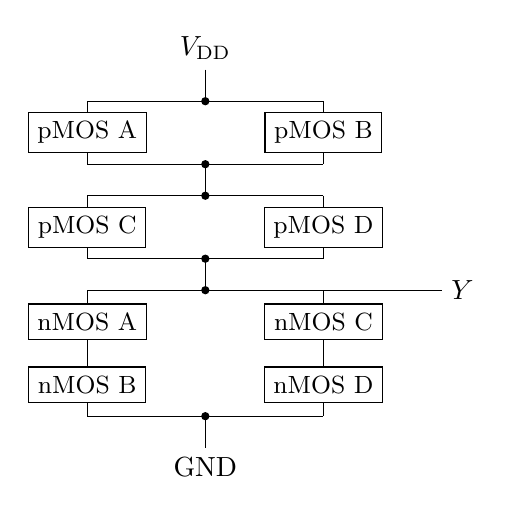
\begin{tikzpicture}[x=1cm,y=0.8cm]
\node[above] at (0,6) {$V_{\mathrm{DD}}$};
\draw (0,6)--(0,5.5)--(-1.5,5.5) (0,5.5)--(1.5,5.5);
\draw (-1.5,5.5)--(-1.5,4.5) node[midway,draw,fill=white,font=\small] {pMOS A};
\draw (1.5,5.5)--(1.5,4.5) node[midway,draw,fill=white,font=\small] {pMOS B};
\draw (-1.5,4.5)--(1.5,4.5);\draw (0,4.5)--(0,4)--(-1.5,4) (0,4)--(1.5,4);
\draw (-1.5,4)--(-1.5,3) node[midway,draw,fill=white,font=\small] {pMOS C};
\draw (1.5,4)--(1.5,3) node[midway,draw,fill=white,font=\small] {pMOS D};
\draw (-1.5,3)--(1.5,3);\draw (0,3)--(0,2.5)--(3,2.5) node[right] {$Y$};
\draw (0,2.5)--(-1.5,2.5)--(-1.5,1.5) node[midway,draw,fill=white,font=\small] {nMOS A};
\draw (0,2.5)--(1.5,2.5)--(1.5,1.5) node[midway,draw,fill=white,font=\small] {nMOS C};
\draw (-1.5,1.5)--(-1.5,0.5) node[midway,draw,fill=white,font=\small] {nMOS B};
\draw (1.5,1.5)--(1.5,0.5) node[midway,draw,fill=white,font=\small] {nMOS D};
\draw (-1.5,0.5)--(1.5,0.5);\draw (0,0.5)--(0,0) node[below] {GND};
\foreach \x/\y in {0/5.5,0/4.5,0/4,0/3,0/2.5,0/0.5} {\fill (\x,\y) circle (1.5pt);}
\end{tikzpicture}
\end{latin}
\caption{نمای توپولوژی آموزشی \lr{AOI22} برای رابطه \eqref{eq:ch1-aoi}.
بلوک‌های برچسب‌دار در این نمایش جایگزین نماد ترانزیستورند؛
وضعیت هدایت هر بلوک به نوع ترانزیستور و ورودی نوشته‌شده در آن بستگی دارد.}
\label{fig:ch1-aoi}
\end{figure}

نام \lr{AND-OR-Invert (AOI22)} می‌گوید دو گروه \lr{AND} دوورودی داریم،
خروجی آن‌ها \lr{OR} و سپس معکوس می‌شود.
در مثال \((A,B,C,D)=(1,1,0,0)\)، شاخه \(AB\) پایین وصل است؛
در بالا گروه \(A,B\) کاملاً قطع است، پس \(Y=0\).
در \((1,0,1,0)\)، هر شاخه پایین یک ترانزیستور قطع دارد؛
در بالا از \(B\) و \(D\) مسیر کامل داریم، پس \(Y=1\).
این دو مثال جای بررسی تمام حالت‌ها را نمی‌گیرند؛ رابطه مکمل، پوشش همه حالت‌ها را می‌دهد.

\textbf{مثال کتاب، \lr{OAI31}.} برای
\(Y=\overline{(A+B+C)D}\)، پایین گروه موازی \(A,B,C\) را با \(D\) سری می‌کنیم.
بالا گروه سری سه \lr{pMOS} با کنترل \(A,B,C\) را با یک \lr{pMOS} کنترل‌شده با \(D\)
موازی می‌کنیم؛ چون شرط بالا
\(\overline{A}\,\overline{B}\,\overline{C}+\overline{D}\) است.
این هشت ترانزیستور، تابع مثال \secnum{۱.۲} کتاب را می‌سازند
\cite[صفحه چاپی ۱۲]{weste}.

\subsection{چرا \lr{AND} را با یک \lr{NAND} و یک \lr{Inverter} می‌سازیم؟}
در خانواده محدود شبکه‌های مکمل ایستا که ورودی‌های غیرمعکوس مستقیماً
\lr{Gate}ها را کنترل می‌کنند، روشن شدن مسیر پایین خروجی را صفر می‌کند؛
ازاین‌رو گیت یک‌مرحله‌ای، تابع معکوس‌کننده ورودی‌هاست.
جابه‌جا کردن ساده \lr{nMOS} و \lr{pMOS} برای ساخت \lr{Buffer} مناسب نیست؛
با انتقال سطوح ضعیف روبه‌رو می‌شویم \cite[صفحه چاپی ۱۴]{weste}.
به‌جای آن، دو معکوس‌سازی می‌دهند
\[
 Y=\overline{\overline{AB}}=AB.
\]
برای \lr{OR} نیز \lr{NOR} و سپس \lr{Inverter} به کار می‌رود.

\lr{AND} دوورودی با این روش شش ترانزیستور دارد: چهار برای \lr{NAND}
و دو برای \lr{Inverter}. ساخت تابع \lr{AOI22} از دو \lr{AND}، یک \lr{OR}
و یک \lr{Inverter} با این سلول‌های ساده، \(6+6+6+2=20\)
ترانزیستور می‌خواهد؛ گیت \lr{Compound} فقط هشت ترانزیستور دارد.
این مقایسه شمارش قطعات است؛ برای نتیجه قطعی درباره \lr{Delay} یا توان باید
اندازه ترانزیستورها، بار و مسیرها نیز تحلیل شوند \cite[شکل \secnum{۱.۲۴}]{weste}.

\subsection{کنترل اعتبار گیت ایستا}
برای هر ترکیب ورودی، ابتدا قطع یا وصل بودن تک‌تک قطعات و سپس وجود مسیر کامل
را مشخص می‌کنیم. اگر پایین هدایت دارد، بالا باید قطع باشد و برعکس.
این کنترل برای تمام ورودی‌ها، شرط منطقی طراحی است.
در مدل ایدئال پایدار، ابعاد ترانزیستورها جدول درستی را عوض نمی‌کنند؛
در مدار واقعی، ابعاد بر زمان و توان و رفتار گذرا اثر دارند.
عبارت «توان ساکن صفر» نیز فقط به مدل بدون نشتی و ورودی‌های پایدار معتبر تعلق دارد؛
بار خازنی و هدایت هم‌زمان در گذار، همچنان انرژی مصرف می‌کنند.
